\chapter{Zwei gekoppelte getriebene harmonische Oszillatoren}


In diesem Teil der Arbeit werden mit Hilfe der aus (\ref{lsg_einzelner}) bekannten Lösung des einzelnen getrieben Oszillators die Wellenfunktionen für ein System hergeleitet, das aus zwei gekoppelten Oszillatoren $x_1$ und $x_2$ der gleichen Masse $m$ besteht, von denen einer mit der periodischen Kraft $S(t) = S(t+T)$ angetrieben wird.
Die Potentialkonstanten $k$ der beiden Oszillatoren sind ebenfalls identisch, aber im Allgemeinen unterschiedlich zur Kopplungskonstante $\kappa$ zwischen den Oszillatoren.
Der Hamilton-Operator dieses Systems kann direkt aus der Hamilton-Funktion  der klassichen Mechanik übernommen werden:
\begin{equation}
  H(t) = H(t+T) = \frac{p_1^2}{2m} + \frac{p_2^2}{2m} + \frac 1 2 kx_1^2 + \frac 1 2 kx_2^2 + \frac 1 2 \kappa(x_2-x_1)^2 - S(t)x_1 \; .
  \label{H_gekoppelt}
\end{equation}
Es werden auch die Erwartungswerte für  den Ort $\braket{x_{1,2}}_{n,l}$ und den Impuls $\braket{p_{1,2}}_{n,l}$, genauso wie der Erwartungswert der Energie $\braket{H}_{n,l}$ und dessen zeitliches Mittel $\bar{H}_{n,l}$ berechnet, indem auf die bekannten Erwartungswerte des einzelnen getriebenen Oszillators zurückgeführt wird.
Die Erwartungswerte werden auch graphisch dargestellt.

Zur Lösung des Systems wird eine unitäre Koordinatentransformation eingeführt, welche den Hamilton-Operator $H(x_1,x_2,p_1,p_2,t)$ zu zwei in den neuen Koordinaten unabhängigen Hamilton-Operatoren $H_+(x_+,p_+,t)$ und $H_-(x_-,p_-,t)$ mit effektiven Potentialkonstanten $k_+,k_-$ entkoppelt, welche je einen einzelnen (getriebenen) Oszillator beschreiben.
Dann ergeben sich die Wellenfunktionen leicht aus denen des einzelnen Oszillators.


%war vorher subsection
\section{Die Schrödinger-Gleichung mit unabhängigen Hamilton-Operatoren}
  Liegt ein Hamilton-Operator der Form
  \begin{equation}
    H = \sum_i H_i(x_i,p_i,t) \;,\; H_i : \cal H_i \rightarrow H_i
    \label{unabh_H}
  \end{equation}
  vor, führt der Ansatz
  \begin{equation}
    \Psi = \prod_i \Psi(x_i,p_i,t) \; , \; \Psi_i \in \cal H_i
    \label{lsg_unabh_H}
  \end{equation}
  auf unabhängige Schrödinger-Gleichungen für die einzelnen Wellenfunktionen \\ $\Psi_i(x_i,p_i,t)$, sodass %\cite{online quelle}
  \begin{equation}
    \text i \hbar \frac{\partial}{\partial t}\Psi_i = \delta_{i,j}  H_j \Psi_i
    \label{schroedglg_unabh_H}
  \end{equation}
  erfüllt ist.
  Um dies schnell zu zeigen, schauen wir uns den Fall von zwei unabhängigen Operatoren an:
  \begin{align}
    \begin{split}
      \text i \hbar \frac{\partial}{\partial t} \Psi = H\Psi \iff \Psi_2 H_1 \Psi_1 + \Psi_1 H_2 \Psi_2 = \text i \hbar \left(\frac{\partial}{\partial t} \Psi_1\Psi_2 + \Psi_1\frac{\partial}{\partial t} \Psi_2 \right) \; .
    \end{split}
  \end{align}
  Da die Operatoren nur auf Funktionen wirken, die auf dem selben Raum definiert sind, kann man sie an der jeweils anderen Funktion vorbei ziehen.
  Wenn wir weiterhin durch unseren Ansatz $\Psi_1\Psi_2$ teilen, wird die Gleichung zu:
  \begin{equation}
    \frac{1}{\Psi_1}H_1\Psi_1 + \frac{1}{\Psi_2}H_2\Psi_2 = \text i \hbar \left(\frac{\frac{\partial}{\partial t} \Psi_1}{\Psi_1} + \frac{\frac{\partial}{\partial t} \Psi_2}{\Psi_2} \right) \; .
  \end{equation}
  Weil die linke und rechte Seite für alle unabhängigen $x_1,p_1,x_2,p_2$ gleich sein müssen, folgen die einzelnen Schrödinger-Gleichungen für die Wellenfunktionen $\Psi_1$ und $\Psi_2$:
  \begin{equation}
    \frac{1}{\Psi_1}H_1\Psi_1 = \frac{\frac{\partial}{\partial t} \Psi_1}{\Psi_1} \; , \; \frac{1}{\Psi_2}H_2\Psi_2 = \frac{\frac{\partial}{\partial t} \Psi_2}{\Psi_2} \; .
  \end{equation}
  Wie an diesem Beispiel zu sehen, gilt Gleiches auch für beliebig viele unabhängige Hamilton-Operatoren, womit (\ref{schroedglg_unabh_H}) erfüllt ist und wir wissen, dass die Lösung $\Psi$ die Form (\ref{lsg_unabh_H}) hat.
  %nur EINE moegliche lsg hat die form psi, wenn wir einschraenken, dass psi so aussehen soll, wer weis ob es noch andere lsgen nicht dieser form gibt.



\section{Unitäre Variablentransformation und allgemeine Lösung der Schrödinger-Gleichung}
  Um für unseren Hamilton-Operator $H(x_1,x_2,p_1,p_2,t)$ (\ref{H_gekoppelt}) eine entkoppelte Form $H(x_+,x_-,p_+,p_-,t)=H_+(x_+,p_+,t)+H_-(x_-,p_-,t)$ nach (\ref{unabh_H}) in den neuen Koordinaten/Variablen $x_+,x_-,p_+,p_-$ zu erhalten, wählen wir die unitären Koordinationtransformationen \cite{arxiv}
  \begin{equation}
    x_+ = \frac{1}{\sqrt{2}}(x_2+x_1) \;,\; x_-=\frac{1}{\sqrt{2}}(x_2-x_1) \;,
    \label{koord_trafo_x}
  \end{equation}
  welche aus den Normalmoden des klassischen Problems folgen, worauf in Kapitel () genauer eingegangen wird.
  Durch einfaches Umstellen folgen $x_1$ und $x_2$ in Abhängigkeit der neuen Koordinaten $x_+$ und $x_-$:
  \begin{equation}
    x_1=\frac{1}{\sqrt{2}}(x_+-x_-) \;,\; x_2=\frac{1}{\sqrt{2}}(x_++x_-) \; .
  \end{equation}
  Indem wir $x_1$ und $x_2$ so im Hamilton-Operator (\ref{H_gekoppelt}) ersetzen, formen wir den ortsabhängigen Teil um zu
  \begin{align}
    &\frac{1}{2}kx_1^2+\frac{1}{2}kx_2^2+\frac{1}{2}\kappa(x_2-x_1)^2-S(t)x_1= \notag\\
    &\frac{1}{2}kx_+^2+\frac{1}{2}(k+2\kappa)x_-^2-S(t)\frac{1}{\sqrt{2}}(x_+-x_-) \; .
  \end{align}
  Es tauchen nun keine Kopplungsterme $x_+x_-$ mehr auf, wie es in den alten Koordinaten der Fall war.

  Jetzt betrachten wir die neuen Impulse und überprüfen, dass es durch den Variablenwechsel nicht zu neuen Kopplungstermen in den $p_+$,$p_-$ kommt.
  Mit der Kettenregel folgt für die Ableitungen der Impulsoperatoren
  \begin{align}
    \frac{\partial}{\partial x_{\pm}} = \frac{\partial}{\partial x_1}\frac{\partial x_1}{\partial x_{\pm}} + \frac{\partial}{\partial x_2}\frac{\partial x_2}{\partial x_{\pm}}
    =\frac{\partial}{\partial x_1}\left(\pm\frac{1}{\sqrt{2}}\right)
    + \frac{\partial}{\partial x_2}\frac{1}{\sqrt{2}}
    = \frac{1}{\sqrt{2}}\left(\frac{\partial}{\partial x_2}\pm\frac{\partial}{\partial  x_1}\right) \;,
  \end{align}
  weshalb für die Impulsoperatoren identisch zu den Ortsoperatoren gilt
  \begin{equation}
    p_+ = \frac{1}{\sqrt{2}}(p_2+p_1) \;,\; p_-=\frac{1}{\sqrt{2}}(p_2-p_1) \; .
    \label{koord_trafo_p}
  \end{equation}
  Wir setzen erneut in unseren Hamilton-Operator (\ref{H_gekoppelt}) ein und erhalten für den impulsabhängigen Teil
  \begin{equation}
    \frac{p_1^2}{2m} + \frac{p_2^2}{2m} = \frac{p_+^2}{2m} + \frac{p_-^2}{2m} \; .
    \label{koord_trafo_p^2}
  \end{equation}

  Wie erwartet bleibt die Summe der quadrierten Impulsoperatoren unverändert.

  Der gesamte Hamilton-Operator der zwei gekoppelten getrieben Oszillatoren ist in den neuen Variablen folglich
  \begin{align}
    H(t) &= H(t+T) = \frac{p_1^2}{2m} + \frac{p_2^2}{2m} + \frac 1 2 kx_1^2 + \frac 1 2 kx_2^2 + \frac 1 2 \kappa(x_2-x_1)^2 - S(t)x_1 \notag\\
    &= \frac{p_+^2}{2m}+\frac{1}{2}kx_+^2-\frac{1}{\sqrt{2}}S(t)x_+ \quad + \quad
    \frac{p_-^2}{2m}+\frac{1}{2}(k+2\kappa)x_-^2+\frac{1}{\sqrt{2}}S(t)x_- \notag\\
    &= \frac{p_+^2}{2m}+\frac{1}{2}k_+x_+^2-S_+(t)x_+ \quad \;\: + \quad
    \frac{p_-^2}{2m}+\frac{1}{2}k_-x_-^2-S_-(t)x_- \notag\\
    &= H_+(x_+,p_+,t) + H_-(x_-,p_-,t) \;,\; H_\pm:\cal H_\pm \rightarrow \cal H_\pm \; .
    \label{gekoppelte_H_entkoppelt}
  \end{align}
  Der Hamilton-Operator in den neuen Variablen $x_{\pm},p_{\pm}$ beschreibt demnach ein System aus zwei unabhängigen getriebenen harmonischen Oszillatoren mit neuen Potentialkonstanten $k_1=k$ und $k_2=k+2\kappa$ bzw. neuen Eigenfrequenzen
  \begin{equation}
    w_+=\sqrt{\frac{k}{m}} \quad\text{und}\quad \omega_-=\sqrt{\frac{k+2\kappa}{m}} \; .
    \label{neue_eigenfrequenzen}
  \end{equation}
  Die beiden Oszillatoren werden, wegen dem verschiedenen Vorzeichen von $S_+(t)=S_+(t+T)$ und $S_-(t)=S_-(t+T)$, periodisch aber phasenversetzt um $\pi$ mit der ursprünglichen Treibkraft $S(t)$ angetrieben, wobei diese mit dem Faktor $1/\sqrt{2}$ skaliert wird.

Betrachten wir den Fall, dass beide Oszillatoren $x_1$ und $x_2$ des Systems in den alten Koordinaten getrieben sind, und zwar genau wie durch die neuen Koordinaten $x_+$ und $x_-$ vorgegeben, das heißt
  \begin{align}
      &H(t) = \frac{p_1^2}{2m} + \frac{p_2^2}{2m} + \frac 1 2 kx_1^2 + \frac 1 2 kx_2^2 + \frac 1 2 \kappa(x_2-x_1)^2 - S(t)(x_2+x_1) \notag\\
      \text{oder} \; &H(t) = \frac{p_1^2}{2m} + \frac{p_2^2}{2m} + \frac 1 2 kx_1^2 + \frac 1 2 kx_2^2 + \frac 1 2 \kappa(x_2-x_1)^2 - S(t)(x_2-x_1) \;,
  \end{align}
  liegt in den neuen Variablen ein vereinfachtes System vor, bei dem nur ein Oszillator $x_+$ oder $x_-$ getrieben ist.
  Es muss also in den klassischen Normalmoden getrieben werden, damit nach dem Variablenwechsel ein möglichst einfaches System mit nur noch einem getriebenen Oszillator vorliegt.

  \textbf{L"osung der Schr"odinger-Gleichung}

  Nach den Ergebnissen dieses und des vorherigen Abschnittes k"onnen wir nun die Wellenfunktion $\Psi_{n,l}(x_1,x_2,p_1,p_2,t)$ des Systems zweier gekoppelter getriebener Oszillatoren (\ref{H_gekoppelt}), f"ur eine allgemeine Treibkraft $S(t)=S(t+T)$, in den neuen entkoppelten Koordinaten $x_+$ und $x_-$, nach Formel (\ref{schroedglg_unabh_H}) hinschreiben.
  Durch Ersetzen der neuen Variablen nach Formel (\ref{koord_trafo_x}) und (\ref{koord_trafo_p^2}) ist auch die Wellenfunktion in den alten Variablen bekannt:
  \begin{align}
     &\Psi_{n,l}(x_+,x_-,t) = \Psi_{+,n}(x_+,t)\Psi_{-,l}(x_-,t) \notag\\
     &=N_{n,+}O_n\left(\sqrt{\frac{m\omega_+}{\hbar}}(x_+-\zeta_+(t))\right) \exp\left(\frac{-m\omega_+}{2\hbar}(x_+-\zeta_+(t))^2\right)\notag\\
     &\quad \cdot \exp\left[\frac{\text i}{\hbar}\left(m\dot \zeta(t)(x_+-\zeta_+(t))-E_{+,n}t+\int_0^tL_+\:\text dt'\right)\right] \quad\quad\quad\notag\\
     &\quad \cdot N_{l,-}O_l\left(\sqrt{\frac{m\omega_-}{\hbar}}(x_--\zeta_-(t))\right) \exp\left(\frac{-m\omega_-}{2\hbar}(x_--\zeta_-(t))^2\right)\notag\\
     &\quad \cdot \exp\left[\frac{\text i}{\hbar}\left(m\dot \zeta(t)(x_--\zeta_-(t))-E_{-,l}t+\int_0^tL_-\:\text dt'\right)\right] \;,\; \Psi_\pm \in \cal H_\pm \notag\\
    &= N_{+,n}N_{-,l} O_n\left(\sqrt{\frac{m\omega_+}{\hbar}}\left(\frac{1}{\sqrt{2}}(x_2+x_1)-\zeta_+(t)\right)\right)O_l\left(\sqrt{\frac{m\omega_-}{\hbar}}\left(\frac{1}{\sqrt{2}}(x_2-x_1)-\zeta_-(t)\right)\right) \notag\\
    &\quad\cdot \exp\left[\frac{-m}{2\hbar}\left(\omega_+\left(\frac{1}{\sqrt{2}}(x_2+x_1)-\zeta_+(t)\right)^2 + \omega_-\left(\frac{1}{\sqrt{2}}(x_2-x_1)-\zeta_-(t)\right)^2\right)\right] \notag\\
    &\quad\cdot \exp\left[\frac{\text i}{\hbar} \left(m\zeta_+(t)\left(\frac{1}{\sqrt{2}}(x_2+x_1)-\zeta_+(t)\right) + m\zeta_-(t)\left(\frac{1}{\sqrt{2}}(x_2-x_1)-\zeta_-(t)\right)\right) \right] \notag\\
    &\quad\cdot \exp \left[\frac{\text i}{\hbar}\left(-(E_{+,n}+E_{-,l})+\int_0^tL_++L_-\:\text dt'\right)\right] \notag\\
    &=\Psi_{n,l}(x_1,x_2,t) \; , \; n,l \in \mathbb N_0 \; .
  \end{align}
  HIER GUCKEN, OB SO AUFSCHREIBEN OK (GEHT UEBER RAND) UND EVTL AUCH IN X1 X2 AUSGESCHRIEBEN (WAHRSCHEINLICH SCHON, DANN AUCH MIT (t) UEBERALL)
  Die klassischen L"osungen $\zeta_\pm$ und die Lagrange-Funktionen $L_\pm$ sind wie bei der L"osung des einzelnen Oszillators bestimmt "uber (\ref{dgl_zeta}) und (\ref{lagrange_zeta}).
  Genauso sind die Normierungskonstanten $N_{+,n}/N_{-,l}$ und ungetriebenen Eigenenergien $E_{+,n}/E_{-,l}$ wie beim einzelnen getriebenen Oszillator definiert, nur die Eigenfrequenz $\omega_0$ wird ersetzt durch die neuen Eigenfrequenzen $\omega_+,\omega_-$ (\ref{neue_eigenfrequenzen}).

  Wie in Abschnitt  beschrieben, ist $\Psi$ in den neuen Variablen das Produkt aus den unabh"angigen Wellenfunktionen $\Psi_+$ und $\Psi_-$, welche L"osungen der einzelnen Schro"dinger-Gleichungen mit $H_+/H_-$ sind, dadurch ist $\Psi$ auch auf dem Raum, das hei"st auf $x_\pm \in (-\infty,\infty)$, normiert, wie am Anfang von Kapitel (\ref{3}) gezeigt:
  \begin{align}
    &\int_{-\infty}^{\infty}\int_{-\infty}^{\infty} |\Psi_{n,l}(x_1,x_2,t)|^2 \: \text dx_1\text dx_2
    =\int_{-\infty}^{\infty}\int_{-\infty}^{\infty} |\Psi_{n,l}(x_+,x_-,t)|^2 \: \text dx_+\text dx_- \notag\\
    &=\int_{-\infty}^{\infty} |\Psi_{+,n}(x_+,t)|^2 \: \text dx_+ \int_{-\infty}^{\infty} |\Psi_{-,l}(x_-,t)|^2 \: \text dx_-
    = 1 \cdot 1 = 1 \; .
    \label{norm_gekoppelt}
  \end{align}

  In den urspr"unglichen Koordinaten sind Kopplungsterme $x_1x_2$ in der Wellenfunktion vorhanden, durch die Hermit-Polynome $O_n/O_l$ treten hierbei im Allgemeinen unterschiedliche Potenzen der $x_1$ und $x_2$ auf.

  Die Floquet-Moden $\Phi_{n,l}(x_+,x_-,t)=\Pshi_+(x_+,t)\Phi_-(x_-,t)$ sind in den neuen Koordinaten das Produkt aus den einzelnen Floquet-Moden (\ref{floquet_moden_einzelner}), so wie die Wellenfunktionen,
  Die Quasienergien sind dadurch die Summe der einzelnen Quasienergien (\ref{epsilon_einzelner}): $\epsilon_{n,l}=\epsilon_{+,n}+\epsilon_{-,l}$.


\section{Erwartungswerte}
  \label{erwartungswerte_gekoppelt}
  Um die Erwartungswerte f"ur die Observablen $x_1,x_2,p_1,p_2$ zu evaluieren, verwenden wir die benutzten Tranformationen f"ur den Ort (\ref{koord_trafo_x}) und den Impuls (\ref{koord_trafo_p}), mit welchen wir die Berechnung auf die schon bekannten Erwartungswerte des einzelnen getriebenen Oszillators zur"uckf"uhren k"onnen.

  Es werden alle Erwartungswerte f"ur eine allgemeine $T$-periodische Treibkraft $S(t)=A\sin(\omega t)$ berechnet und f"ur die konkrete sinusf"ormige Treibkraft aus Kapitel (\ref{epsilon_sinus_kraft}), f"ur einfache Konstanten, visualisiert.

  Die "+" und "-" Operatoren wirken auf verschiedene Variablen/operieren auf den verschiedenen R"aumen $\cal H_+,\cal H_-$.
  Aus diesem Grund gilt f"ur den Erwartungswert eines Operators $U_+:\cal H_+ \rightarrow \cal H_+$ bez"uglich einer Wellenfunktion der Form $\Psi_{n,l}=\Psi_{+,n}\Psi_{-,l}$ mit $\Psi_\pm \in \cal H_\pm$, wegen der Normierung nach Formel (\ref{norm_gekoppelt}):
  \begin{align}
    \braket{U_+}_{n,l} &= \int_{-\infty}^{\infty}\int_{-\infty}^{\infty} \Psi*U_+\Psi \: \text dx_+ \text dx_-
    = \int_{-\infty}^{\infty} |\Psi_-|^2 \: \text dx_- \int_{-\infty}^{\infty} \Psi_{+,n}^*U_+\Psi_{+,n}^* \: \text dx_+ \notag\\
    &= 1 \cdot \braket{U_+}_n^+ \; .
    \label{erwartungswert_gekoppelt}
  \end{align}
  F"ur einen Operator $U_+$ ist Erwartungswert der Gesamtwellenfunktion $\Psi_{n,l}$ der gekoppelten getriebenen Oszillatoren also identisch zum Erwartungswert der Wellenfunktion des einzelnen getriebenen Oszillators, in den "+"-Koordinaten.
  F"ur $U_-$ gilt Gleiches.

  Demnach folgt f"ur den Erwartungswert $\braket{U_+U_-}_{n,l}$
  \begin{equation}
    \braket{U_+U_-}_{n,l}=\braket{U_-U_+}_{n,l} = \braket{U_+}_n^+\braket{U_-}_l^- \; .
    \label{erwartungswert_gekoppelt_produkt}
  \end{equation}


  \subsection{Zeitabh"angige Erwartungswerte des Ortes}
    Mit der Transformation (\ref{koord_trafo_x}), der "Uberlegung zum gekoppelten Erwartungswert (\ref{erwartungswert_gekoppelt}) und dem Erwartungswert des einzelnen getriebenen Oszillators (\ref{erwartungswert_x_einzelner}) aus Kapitel (\ref{3}), sind nun die Erwartungswerte
    $\braket{x_1}_{n,l}/\braket{x_2}_{n,l}$ bekannt:
    \begin{align}
      \braket{x_{1 \atop 2}}_{n,l}=\frac{1}{\sqrt{2}}\left(\braket{x_+}_{n,l}\mp\braket{x_-}_{n,l}\right)
      =\frac{1}{\sqrt{2}}\left(\braket{x_+}_n^+\mp\braket{x_-}_l^-\right)
      =\frac{1}{\sqrt{2}}(\zeta_+(t)\mp\zeta_-(t)) \; .
    \end{align}
    Der Mittelwert des Ortes f"ur einen der beiden Oszillatoren $x_1$ oder $x_2$ des gekoppelten Systems ist somit die quantenzahlunabh"angige Differenz oder die Summe der beiden klassichen L"osungen $\zeta_+$ und $\zeta_-$ der entkoppelten Oszillatoren nach der Variablentransformation, multipliziert mit $1/\sqrt 2$.

    Der Erwartungswert f"ur $x_{1}^2/x_2^2$ ergibt sich dar"uber hinaus mit Formel (\ref{erwartungswert_gekoppelt_produkt}) und zus"atzlich dem Erwartungswert (\ref{erwartungswert_x^2_einzelner}) zu
    \begin{align}
      \braket{x_{1\atop 2}^2}_{n,l}&=\frac{1}{2}\left(\braket{x_+}_{n,l}\pm\braket{x_-}_{n,l}\right)^2
      =\frac{1}{2}\left(\braket{x_+^2}_n^+ \mp 2\braket{x_+}_n^+\braket{x_-}_l^- - \braket{x_-^2}_n^+\right) \notag\\
      &=\frac 1 2 (s_+^2(2n+1)+\zeta_+^2(t) \mp 2\zeta_+(t)\zeta_-(t) + s_-^2(2l+1)\zeta_-^2(t)) \; ,
    \end{align}
    mit $s_\pm$ der charachteristischen L"ange des ungetriebenen OSzillator nach (\ref{charak_laenge}), mit der jeweiligen Eigenfrequenz $\omega_\pm$.

    \textbf{Sinusoidiale Treibkraft}

    F"ur eine sinusoidiale Treibkraft $S(t)=A\sin(\omega t)$ und entsprechenden $S_\pm(t)$ (siehe (\ref{gekoppelte_H_entkoppelt})) sind $\zeta_\pm(t)$ gegeben durch (\ref{zeta_sinuskraft})
    \begin{align}
      \zeta_\pm(t) = \frac{\pm\frac{1}{\sqrt 2} A\sin(\omega t)}{m(\omega_\pm^2 - \omega^2)} \; .
    \end{align}
    %Betrachten wir, wann
    Hiermit werden die Ewartungswerte $\braket{x_1}_{n,l}$ und $\braket{x_2}_{n,l}$, f"ur die Konstanten
    \begin{equation}
      \omega=2 \;,\; A=1 \;,\; k=1 \;,\; m=1 \;,\; \hbar=1 \; ,
    \end{equation}
    dargestellt.
    Hierbei untersuchen wir, f"ur welche Kopplungskonstanten $\kappa$ die beiden Erwartungswerte gleichphasig oder gegenphasig bzw. mit selbem oder unterschiedlichem Vorzeichen der Amplitude schwingen, also bei welchem $\kappa$ die Amplitude $\braket{x_1}_{n,l}$ ihr Vorzeichen "andert.
    Wir betrachten somit die Situation einer schwachen (gegenphasig) und starken (gleichphasig) Kopplung.

    Die Amplitude von $\braket{x_2}_{n,l}$ kann ihr Vorzeichen nicht "andern, da negative Kopplungskonstanten nicht sinnvoll sind, der Erwartungswert verschwindet genau f"ur $\kappa=0$, wie in Abb.(\ref{fig:x2_null}) veranschaulicht.
    Dies entspricht der Erwartung, da es sich bei $x_2$ ohne Kopplung um einen einzelnen ungetriebenen Oszillator handelt, weil nur $x_1$ getrieben ist.

    Der Erwartungswert von $x_1$ wechselt sein Vorzeichen f"ur/ist genau 0 f"ur $\kappa=\omega^2m-k = 2^2\cdot1-1=3$, wie in Abb.(\ref{fig:x1_null}) gezeigt.
    Die gegenphasige (schwache) Kopplung ist f"ur 4$\kappa=1<3$ in Abb.(\ref{fig:schwach}) dargestellt. Wie klassisch anzunehmen, ist die Amplitude des Erwartungswertes $\braket{x_2}_{n,l}$ des angekoppelten Oszillators in diesem Fall geringer als die des getriebenen Oszillator-Erwartungswertes $\braket{x_1}_{n,l}$.
    Die gleichphasige (starke) Kopplung ist f"ur $\kappa=15>3$ in Abb.(\ref{fig:stark}) dargestellt.
    F"ur eine starke Kopplung werden die Erwartungswerte identisch und die Amplitude geringer, was der klassischen Anschauung zweier starr gekoppelter Oszillatoren entspricht.


    \begin{figure}
      \begin{subfigure}[t]{0.5\textwidth}
        \centering
        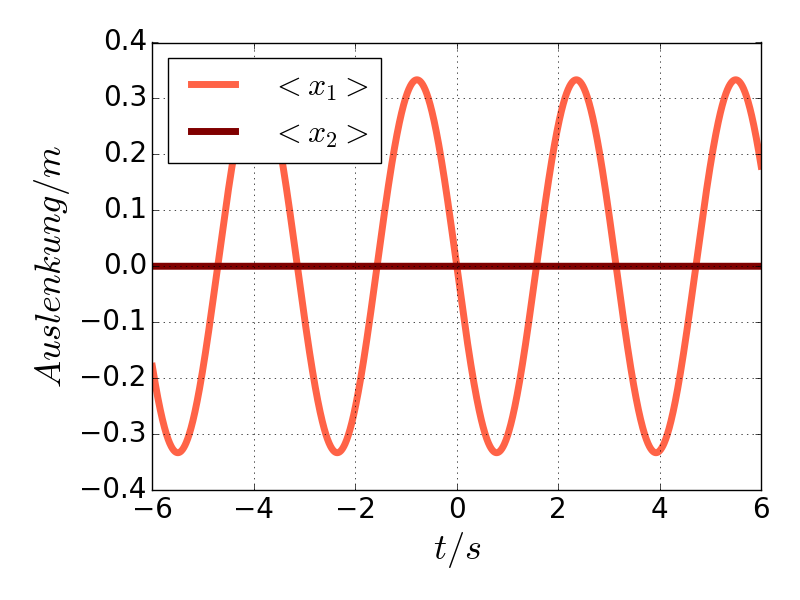
\includegraphics[width=\textwidth]{plots/<x2>nl0.png}
        \caption{$\kappa=0$.}
        \label{fig:x2_null}
      \end{subfigure}
      %\quad
      \begin{subfigure}[t]{0.5\textwidth}
          \centering
          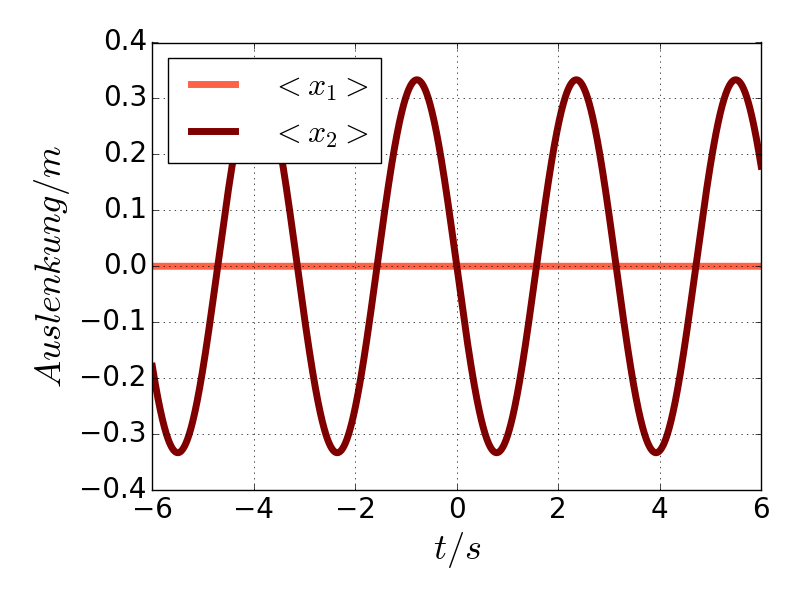
\includegraphics[width=\textwidth]{plots/<x1>nl0.png}
          \caption{$\kappa=3$.}
          \label{fig:x1_null}
      \end{subfigure}
      %\quad
      \begin{subfigure}[t]{0.5\textwidth}
        \centering
        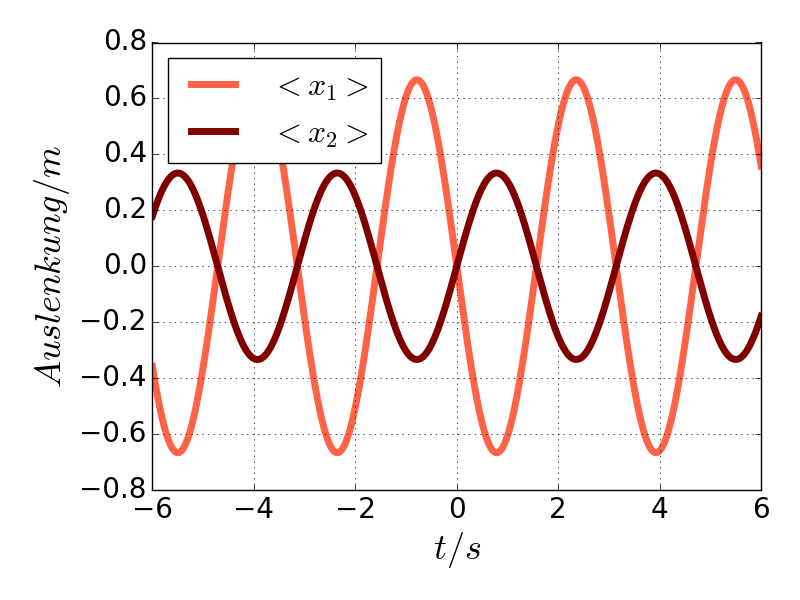
\includegraphics[width=\textwidth]{plots/<x12>nlschwach.png}
        \caption{$\kappa=1$.}
        \label{fig:schwach}
      \end{subfigure}
      %\quad
      \begin{subfigure}[t]{0.5\textwidth}
          \centering
          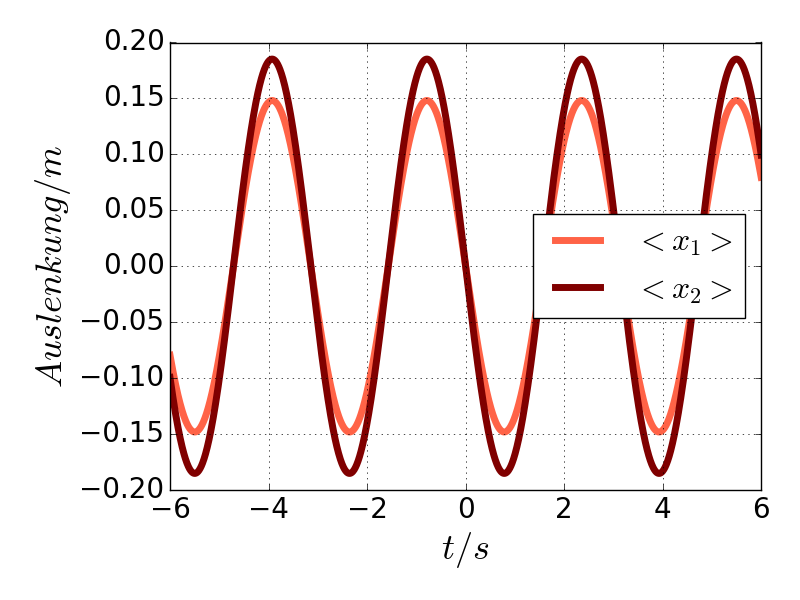
\includegraphics[width=\textwidth]{plots/<x12>nlstark.png}
          \caption{$\kappa=15$.}
          \label{fig:stark}
      \end{subfigure}
      \caption{Erwartungswerte der gekoppelten Oszillatoren $\braket{x_1}_{n,l}$ und $\braket{x_2}_{n,l}$ mit $\omega=2 \;,\; A=1 \;,\; k=1 \;,\; m=1 \;,\; \hbar=1$.}
    \end{figure}

  \subsection{Zeitabh"angige Erwartungswerte des Impulses}
    Die Transformation der Impulsoperatoren (\ref{koord_trafo_p}) hat die gleiche Form wie bei den Ortsoperatoren (\ref{koord_trafo_x}), die Berechnung der Erwartungswerte $\braket{p_{1 \atop 2}}_{n,l}$ und $\braket{p_{1\atop 2}^2}_{n,l}$ erfolgt darum analog, mit den Impuls-Erwartungswerten (\ref{erwartungswert_p_einzelner}) und (\ref{erwartungswert_p^2_einzelner}).
    Es gilt:
    \begin{align}
      \braket{p_{1 \atop 2}}_{n,l}=\frac{1}{\sqrt{2}}\left(\braket{p_+}_{n,l}\mp\braket{p_-}_{n,l}\right)
      =\frac{1}{\sqrt{2}}\left(\braket{p_+}_n^+\mp\braket{p_-}_l^-\right)
      =\frac{m}{\sqrt{2}}(\dot\zeta_+(t)\mp\dot\zeta_-(t)) \;
    \end{align}
    und
    \begin{align}
      \braket{p^2_{1\atop 2}}_{n,l}&=\frac{1}{2}\left(\braket{p_+}_{n,l}\pm\braket{p_-}_{n,l}\right)^2 \notag\\
      %=\frac{1}{2}\left(\braket{p_+^2}_n^+ \mp 2\braket{p_+}_n^+\braket{x_-}_l^- - \braket{x_-^2}_n^+\right) \notag\\
      &=\frac {m^2} 2 (\omega_+^2s_+^2(2n+1)+\ddot\zeta_+^2(t) \mp 2\dot\zeta_+(t)\dot\zeta_-(t) + \omega_-^2s_-^2(2l+1)\ddot\zeta_-^2(t)) \; .
    \end{align}
    Die Erwartungswerte sind "ahnlich zu denen des Ortes, wie beim einzelnen Oszillator kommt nur ein Faktor hinzu und die $zeta_\pm(t)$ werden zu ihren Ableitungen.

    F"ur eine sinusoidiale Treibkraft, sehen die Erwartungswerte fur $p_{1\atop 2}$ demnach so aus wie die $\braket{x_{1\atop 2}}_{n,l}$ nur mit skalierter Amplitude und phasenverschoben um $\pi$.
    Das Verhalten f"ur die verschiedenen $\kappa$ ist ebenfalls identisch.

  \subsection{Erwartungswerte der Energie}
    Der Erwartungswert $\braket{H(t)}_{n,l}$ des Hamilton-Operators f"ur eine beliebige Treibkraft $S(t)$ ist auch mit dem Erwatungswert des einzelnen Oszillators berechenbar, indem wir wieder in den neuen Koordinaten arbeiten:
    \begin{align}
      \braket{H(t)}_{n,l} &= \braket{H_+(t)}_n^+ + \braket{H_-(t)}_l^- \notag\\
      &= E_{+,n}+E_{-,l} -L_+-L_- +m\dot\zeta_+^2(t)+m\dot\zeta_-^2(t) \; .
    \end{align}
    Der mittlere Erwartungswert $\bar H_{n,l}$ wird wieder in den neuen Koordinaten, mit Formel (\ref{mittleres_H}), berechnet.
    Weil die Quasieenergien $\epsilon_{n,l}$ die Summe von $\epsilon_{+,n}$ und $\epsilon_{-,l}$ ist, kriegen wir sofort
    \begin{equation}
      \bar H_{n,l}=\bar H_{+,n}+\bar H_{-,l} \; ,
    \end{equation}

    \textbf{Sinusoidiale Treibkraft}

    F"ur das Beispiel der Sinus-Kraft folgt $\braket{H(t)}_{n,l}$ mit den ensprechenden Orts- und Impulserwartungswerten aus vorherigem Abschnitt und  $\bar{H(t)}_{n,l}$ folgt aus Gleichung (\ref{mittleres_H_sinus}).
    Der Erwartungswert der Energie $\braket{H(t)}_{n,l}$ und dessen zeitliches Mittel $\bar{H(t)}_{n,l}$ sind f"ur die selben Konstanten wie zuvor
    \begin{equation}
      \omega=2 \;,\; A=1 \;,\; k=1 \;,\; m=1 \;,\; \hbar=1 \; ,
    \end{equation}
    in Abb.(\ref{fig:H}) aufgetragen.
    Da beide Erwartungswerte wegen den $E_{+,n}/E_{-,l}$ abh"angig von den Quantenzahlen sind, wird hier der einfachste Fall $n=l=0 \rightarrow E_{\pm,0}=\hbar \omega_\pm/2$ betrachtet.
























































b
